% todo:
% - přidat obrázek vykreslující autokorelace + popis proč máme 5 iterací
% - odkaz na podkapitoly ve výsledcích (konec kapitoly 6.1)
% - KAPITOLA 6.2 - KVALITA obecně
% - najít zdroj mluvící o využití Hjorthových deskriptorů pro kvalitu signálu
% - aktualizovat obrázek 6.1

\chapter{Využití Hjorthových deskriptorů na odhad TF a kvality signálů}
\label{ch:hjorth}
% Důvody použití Hjorthových deskriptorů pro odhad TF.
% - Metoda nevyžaduje identifikaci systolických vrcholů.
% Argumentace robustností vůči šumu a periodicitou PPG signálu.
% Hjorthovy parametry se běžně používají v EEG (např. pro klasifikaci stavů), ale pro TF z PPG je to méně časté - a tedy inovativní.
V této kapitole je popsán alternativní přístup k odhadu srdeční tepové frekvence (\acs{TF}) z fotopletysmografického signálu (\acs{PPG}), využívající Hjorthovy deskriptory (také označované jako Hjorthovy parametry).
Na rozdíl od standardních metod~\cite{ENIKÖ,Charlton2022,NeuroKit2}, které se opírají o detekci jednotlivých systolických vrcholů a výpočet \acs{IBI}, využívá tento přístup frekvenční vlastnosti analyzovaného signálu.
To je výhodou v případech, kdy je signál poškozen šumem, artefakty, nebo když je kladen důraz na výpočetní náročnost a rychlost algoritmu.

V podkapitole~\ref{sec:hjorth_kvalita} je popsán způsob využití Hjorthových deskriptorů pro hodnocení kvality signálu. % extend

Hjorthovy deskriptory představují trojici časových charakteristik, původně zavedených Hjorthem v~roce 1970 pro kvantitativní popis elektroencefalografických (\acs{EEG}) signálů~\cite{Hjorth1973}.
Jedná se o parametry \textit{aktivita} (\(H_0\)), \textit{mobilita} (\(H_1\)) a \textit{komplexita} (\(H_2\)), které odrážejí střední výkon, střední úhlovou frekvenci a šířku pásma.
Jejich výpočet vychází čistě z časové domény a nevyžaduje transformaci do frekvenční oblasti.

V oblasti zpracování \acs{PPG} signálů byly Hjorthovy parametry doposud využívány převážně pro hodnocení kvality signálu a detekci artefaktů~\cite{Peralta2017}. % some more references for quality!
Právě proto je v naší práci navržen a realizován nový způsob odhadu \acs{TF} na základě Hjorthovy \textit{mobility} (\(H_1\)).
Tu počítáme na filtrovaných a několikanásobně autokorelovaných signálech.
Struktura navrženého algoritmu je znázorněna na Obr.~\ref{fig:hjorth_schemata}.

\begin{figure}[h]
	\centering
	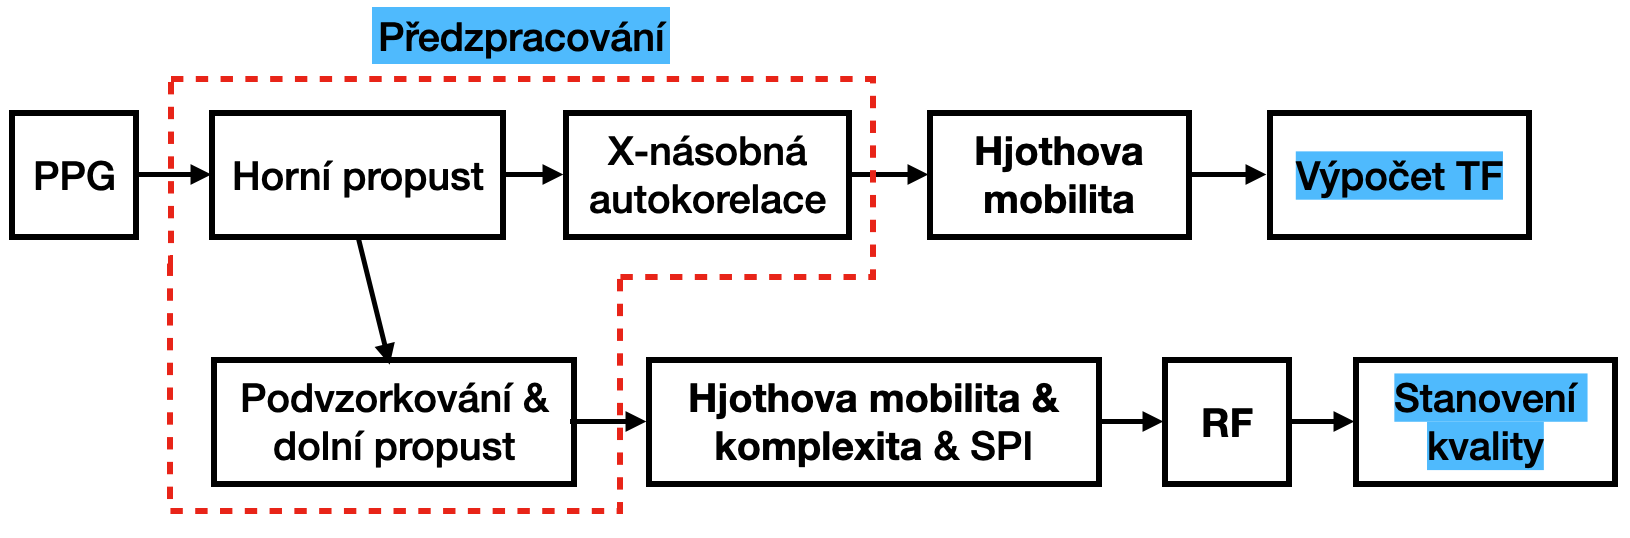
\includegraphics[width=1\textwidth]{./obrazky/hjorth_schema.png} % aktualizovat hodnocení kvality
	\caption[Schéma našeho algorimu, který využívá Hjorthových deskriptorů]{Blokové schéma našeho využití Hjorthových deskriptorů.}
	\label{fig:hjorth_schemata}
\end{figure}

\section{Odhad TF pomocí Hjorthovy mobility}
\label{sec:hjorth_mobilita_tf}
% Načtení signálů z databází probíhá stejně jako u \ref{sec:alg_load}
% Rozdělení signálů je více modulativní, než u \ref{sec:alg_split} pro CapnoBase můžeme použít celý signál nebo libovolný počet oken s maximální délkou odpovídající 10s signálu. Pro BUT PPG (10s signály) to není možné.
Jak již bylo uvedeno, Hjorthova \textit{mobilita} (\( H_1 \)) představuje odhad střední (resp. dominantní) úhlové frekvence signálu v časové oblasti a to bez nutnosti výpočtu Fourierovy transformace.
Tímto způsobem lze efektivně odhadnout frekvenční charakteristiku i v reálném čase, bez transformace do frekvenční oblasti.

Načtení signálů z databází probíhá stejným způsobem jako u našeho prvního algoritmu, popsaného v podkapitole~\ref{sec:alg_load}.
Odlišně jsme však přistoupili k rozdělení signálů.
Zatímco v předchozím algoritmu jsme signály z \textit{CapnoBase} databáze dělili na minutové úseky, zde si můžeme ve vstupu funkce zvolit libovolný počet úseků, na které signál rozdělíme.
Maximální počet těchto úseků odpovídá situaci, kdy jeden úsek trvá 10~s.
Pokud na konci po rozdělení signálu zůstane jeho část, pak je tato část ignorována.

\begin{figure}[t]
	\centering
	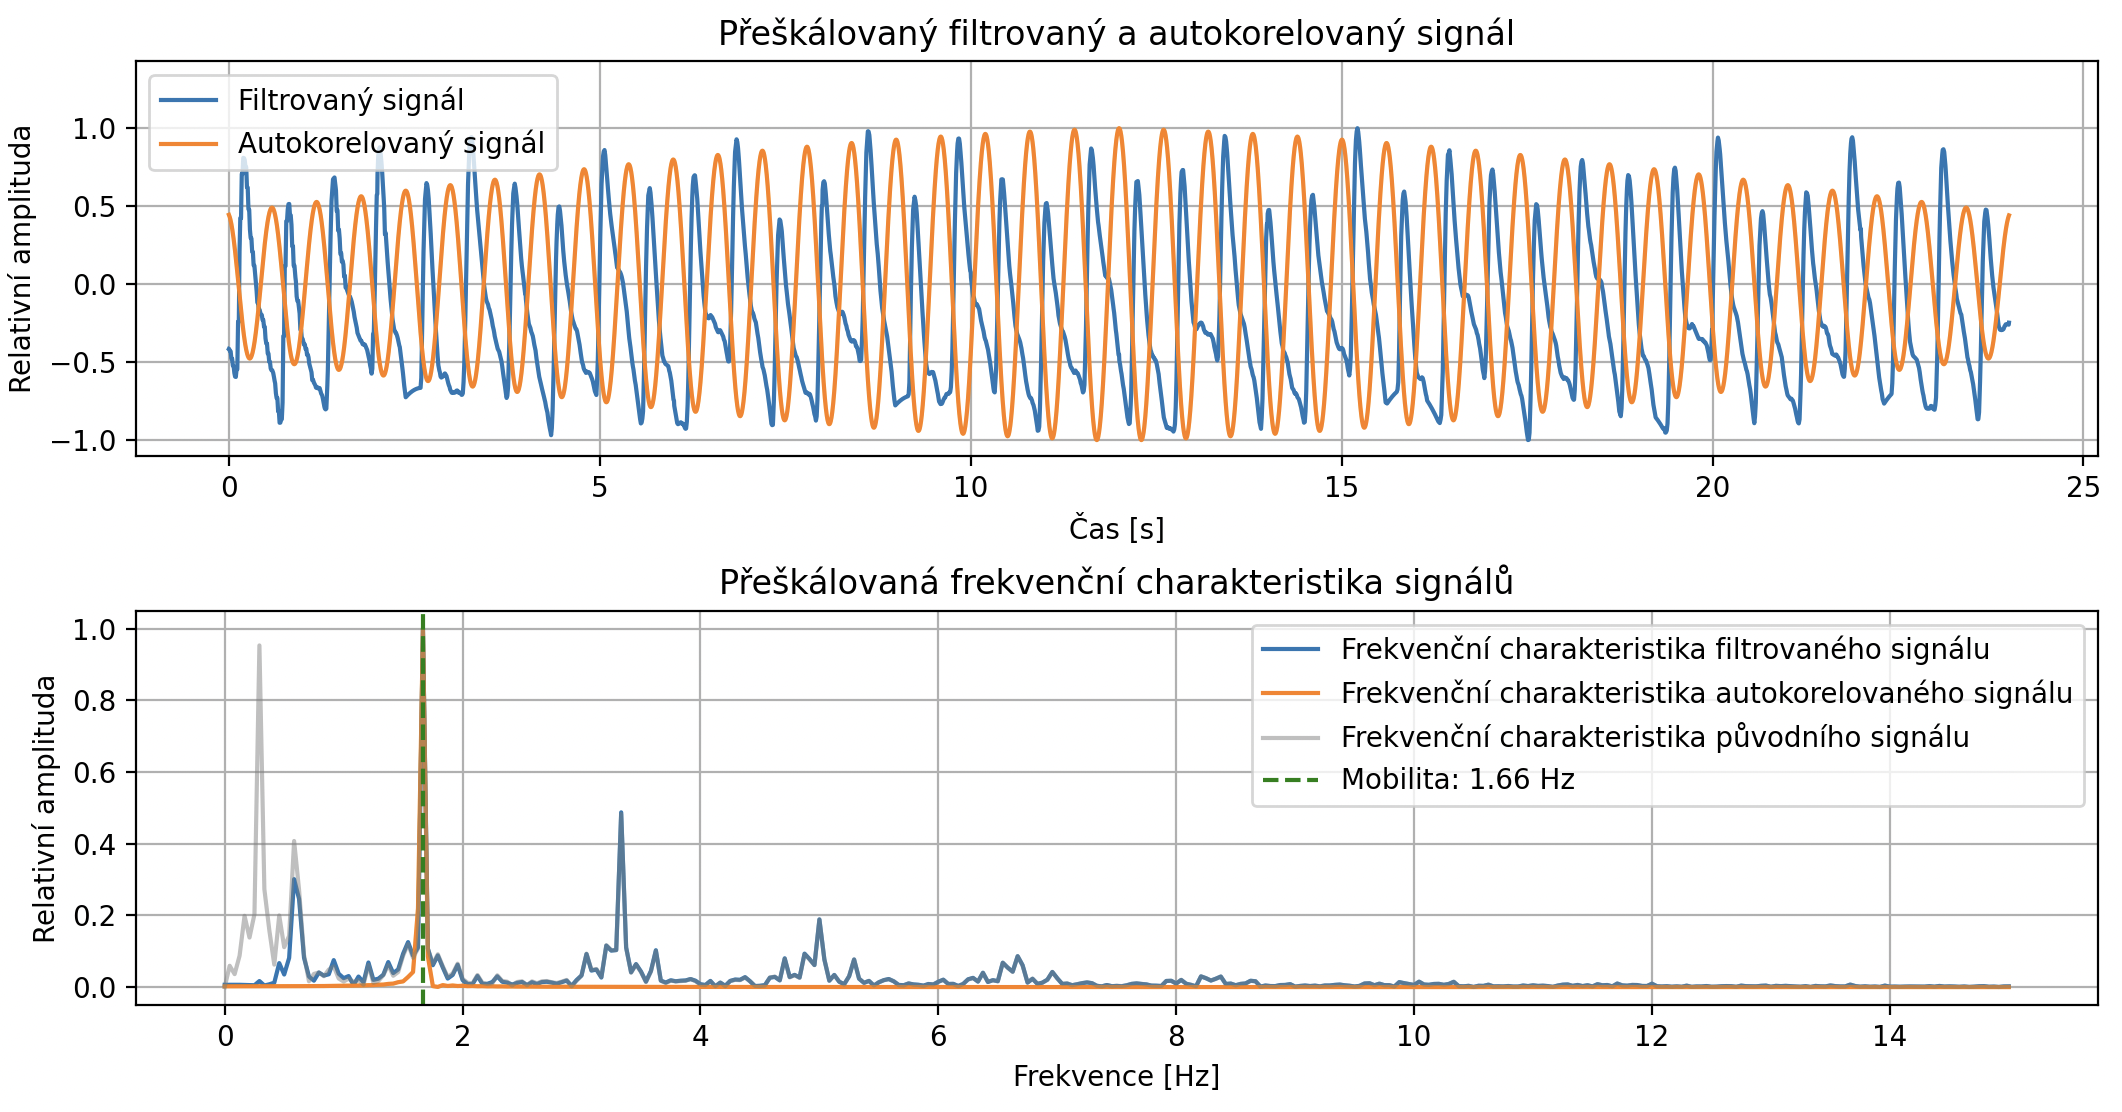
\includegraphics[width=1\textwidth]{./obrazky/hjorth_autocorr_freq.png}
	\caption[Porovnání filtrovaného a autokorelovaného signálu]{Porovnání filtrovaného a autokorelovaného signálu.}
	\label{fig:hjorth_autocorr}
\end{figure}

\subsection*{Předzpracování}
\label{sec:predzpracovani}
% Odstranění stejnosměrné složky signálu -> standardizace signálu.
% High-pass filtraci pro odstranění respirační složky.
% Jak fungiuje vícenásobná autokorelace - cílem je zvýraznění periodické složky.
% Grafy autokorelace, původní signál, frekvenční spektrum obou signálů.
% KEEP IN MIND: Nepotlačují se frekvence, ale složky o vyšších/nižších frekvencích.
Nejprve jsme odstranili stejnosměrnou (\acs{DC}) složku signálu, tedy jeho střední hodnotu \(\mu\).
To jsme učinili proto, aby neovlivňovala výpočet rozptylu signálu a tudíž ani nesnižovala výslednou hodnotu mobility.
Abychom zabránili přetečení data u (\ref{eq:hjorth_var_signal}) a (\ref{eq:hjorth_var_signal_diff}), a zároveň zachovali tvar signálu, vydělili jsme signál bez \( \mu \) jeho směrodatnou odchylkou \( \sigma \).
Rovnice pro standardizaci signálu je následující:
\begin{equation}
	x[n] = \frac{x[n] - \mu}{\sigma}.
\end{equation}

Následně byl signál filtrován hornopropustným filtrem s mezní frekvencí 0,5~Hz, který jsme navrhli k potlačení respirační složky signálu.
Prahová frekvence byla zvolena na základě předpokládané minimální hodnoty \acs{TF}, zmíněné již v podkapitole~\ref{sec:STF}.
Použit byl Butterworthův filtr čtvrtého řádu.

Získaný signál byl dále pětkrát za sebou autokorelován. % 5x, protože to mělo nejlepší výsledky na 10s signálech - vhodné pro porovnání s BUT PPG, ale pro signály z CapnoBase (8min) byly vhodné 3 iterace. Pro 1min signály to bylo zase 4 iterace. Ale pro BUT databázi jsou nejlepší 3 iterace.
Autokorelace je operace, při které se signál koreluje sám se sebou při v různých časových posunech.
Pětinásobná autokorelace byla zvolena na základě \dots. % doplnit
Cílem opakované autokorelace je zvýraznit periodickou strukturu signálu a potlačit nepravidelné nebo náhodné oscilace.
U čistého \acs{PPG} signálů jsou periodické složky rovny systolickým fázím, diastolickým fázím a respiračním složkám.
Klasická autokorelační funkce diskrétního signálu \( x[n] \) je definovaná jako:
\begin{equation}
	r_x[n] = \sum_{k=0}^{N-n-1} x[k] \cdot x[k+n],
\end{equation}
kde \( N \) je délka signálu a \( n \) je zpoždění.
Výpočet v~praxi probíhal ve frekvenčním spektru pomocí rychlé Fourierově transformaci, což snižuje výpočetní náročnost na \( O(i \cdot N \log N) \), kdy \( i \) je počet iterací autokorelace.

Porovnání filtrovaného a autokorelovaného signálu je znázorněno na Obr.~\ref{fig:hjorth_autocorr} společně s jejich frekvenčními charakteristikami a navíc i frekvenční charakteristikou původního signálu.

\subsection*{Výpočet TF z mobility}
\label{sec:TF_mobilita}
% Vysvětlení co znamenajá mobilita a jak se počítá -> vzorec.
% Jak se počítá TF z mobility - vzorec.
% první diference = aproximujeme dva body vedle sebe
Z výsledného signálu po čtvrté iteraci autokorelace jsme vypočítali Hjorthovu mobilitu~\cite{Hjorth1973,Geetika2022}.
Ta je definována jako druhá odmocnina poměru rozptylu první derivace signálu ku rozptylu signálu samotného:
\begin{equation}
	\label{eq:hjorth_mobility}
	H_1 = \sqrt{ \frac{ \mathrm{var}(x[n] - x[n-1]) }{ \mathrm{var}(x[n]) } } = \sqrt{ \frac{ \mathrm{var}(x') }{ \mathrm{var}(x) } } \; [\mathrm{rad/s}].
\end{equation}

Jelikož pracujeme v diskrétním prostředí, derivaci jsme aproximovali pomocí první diference.
Rozptyl signálu \( x \) je definován jako průměr hodnot signálu umocněných na druhou:
\begin{equation}
	\label{eq:hjorth_var_signal}
	\mathrm{var}(x) = \frac{1}{N} \sum_{n=0}^{N-1} (x[n])^2,
\end{equation}
kde \( N \) je délka okna a střední odchylka \( \mu \) je již odečtena v rámci předzpracování, tudíž je rovna nule.
Podobně je definován i rozptyl první derivace signálu \( x' \):
\begin{equation}
	\label{eq:hjorth_var_signal_diff}
	\mathrm{var}(x') = \frac{1}{N} \sum_{n=0}^{N-1} (x[n] - x[n-1])^2.
\end{equation}

Z hodnoty \( H_1 \)~[rad/s] jsme následně odvodili dominantní frekvenci \( f_{dom} \)~[Hz], kterou jsme vynásobili šedesáti, abychom dostali odpovídající hodnotu \acs{TF} v tepech za minutu:

\begin{equation}
	\const{TF}_{\textind{Hjorth}} = 60 \cdot f_{\textind{dom}} = \frac{60 \cdot H_{\textind{1}}}{2\pi}.
\end{equation}

Přestože mají klasické metody detekce vrcholů~\cite{Elgendi2013} lineární průchod signálem se asymptotickou složitostí \( O(N) \), jejich praktická výpočetní náročnost může být vyšší kvůli víceprůchodovým algoritmům, adaptivním prahům, filtrováním nebo nastavování bloků zájmu, jak je uvedeno v podkapitole~\ref{sec:blocks}.
Naopak výpočet Hjorthovy mobility po \( i \) iteracích autokorelace (prováděné pomocí \acs{FFT}) má složitost \( O(i \cdot N \log N) \), avšak díky své jednoduchosti a absenci větvení může být v praxi rychlejší.

Výsledky odhadu \acs{TF} na základě Hjorthovy mobility jsou diskutovány v kapitole~\ref{ch:vysledky}, přičemž porovnání rychlosti exekuce algoritmů je uvedeno v podkapitole XX. % rewrite for specific subsection

\section{Využití mobility a komplexity pro hodnocení kvality signálu}
\label{sec:hjorth_kvalita}
% Vysvětlení co znamenajá mobilita a komplexita a jak se počítají -> vzorec.
% - Mobilita_filtr a Komplexita_filtr
% Vysvětlit jak se počítá SPI
% Jaké prahy jsme nastavili pro hodnocení kvality signálu.